\documentclass[runningheads]{llncs}
%
\usepackage{graphicx}
% Used for displaying a sample figure. If possible, figure files should
% be included in EPS format.
%
% If you use the hyperref package, please uncomment the following line
% to display URLs in blue roman font according to Springer's eBook style:
% \renewcommand\UrlFont{\color{blue}\rmfamily}

\begin{document}
%
\title{Distributed Inventory Manager}

\author{Group 14: Johannes Hartmann \and Luca Schwarz \and Marko Juric}

\institute{}
%
\maketitle              % typeset the header of the contribution

\section{Introduction}

As part of the course project an inventory system shall be developed. The system will be a client server architecture where the servers are responsible to keep the data and process updates regarding goods and stock information. The clients can request the currently available goods and the amount and send update information if new goods are available or if goods are taken out of stock. For the updates it’s important to ensure strong consistency and ordering of events such that all clients have the current information. Within the servers it shall be possible to add additional nodes to the system dynamically and to handle different failure cases while still being able to process requests.


\section{Project Requirements Analysis}



\section{Architecture}

\begin{figure}
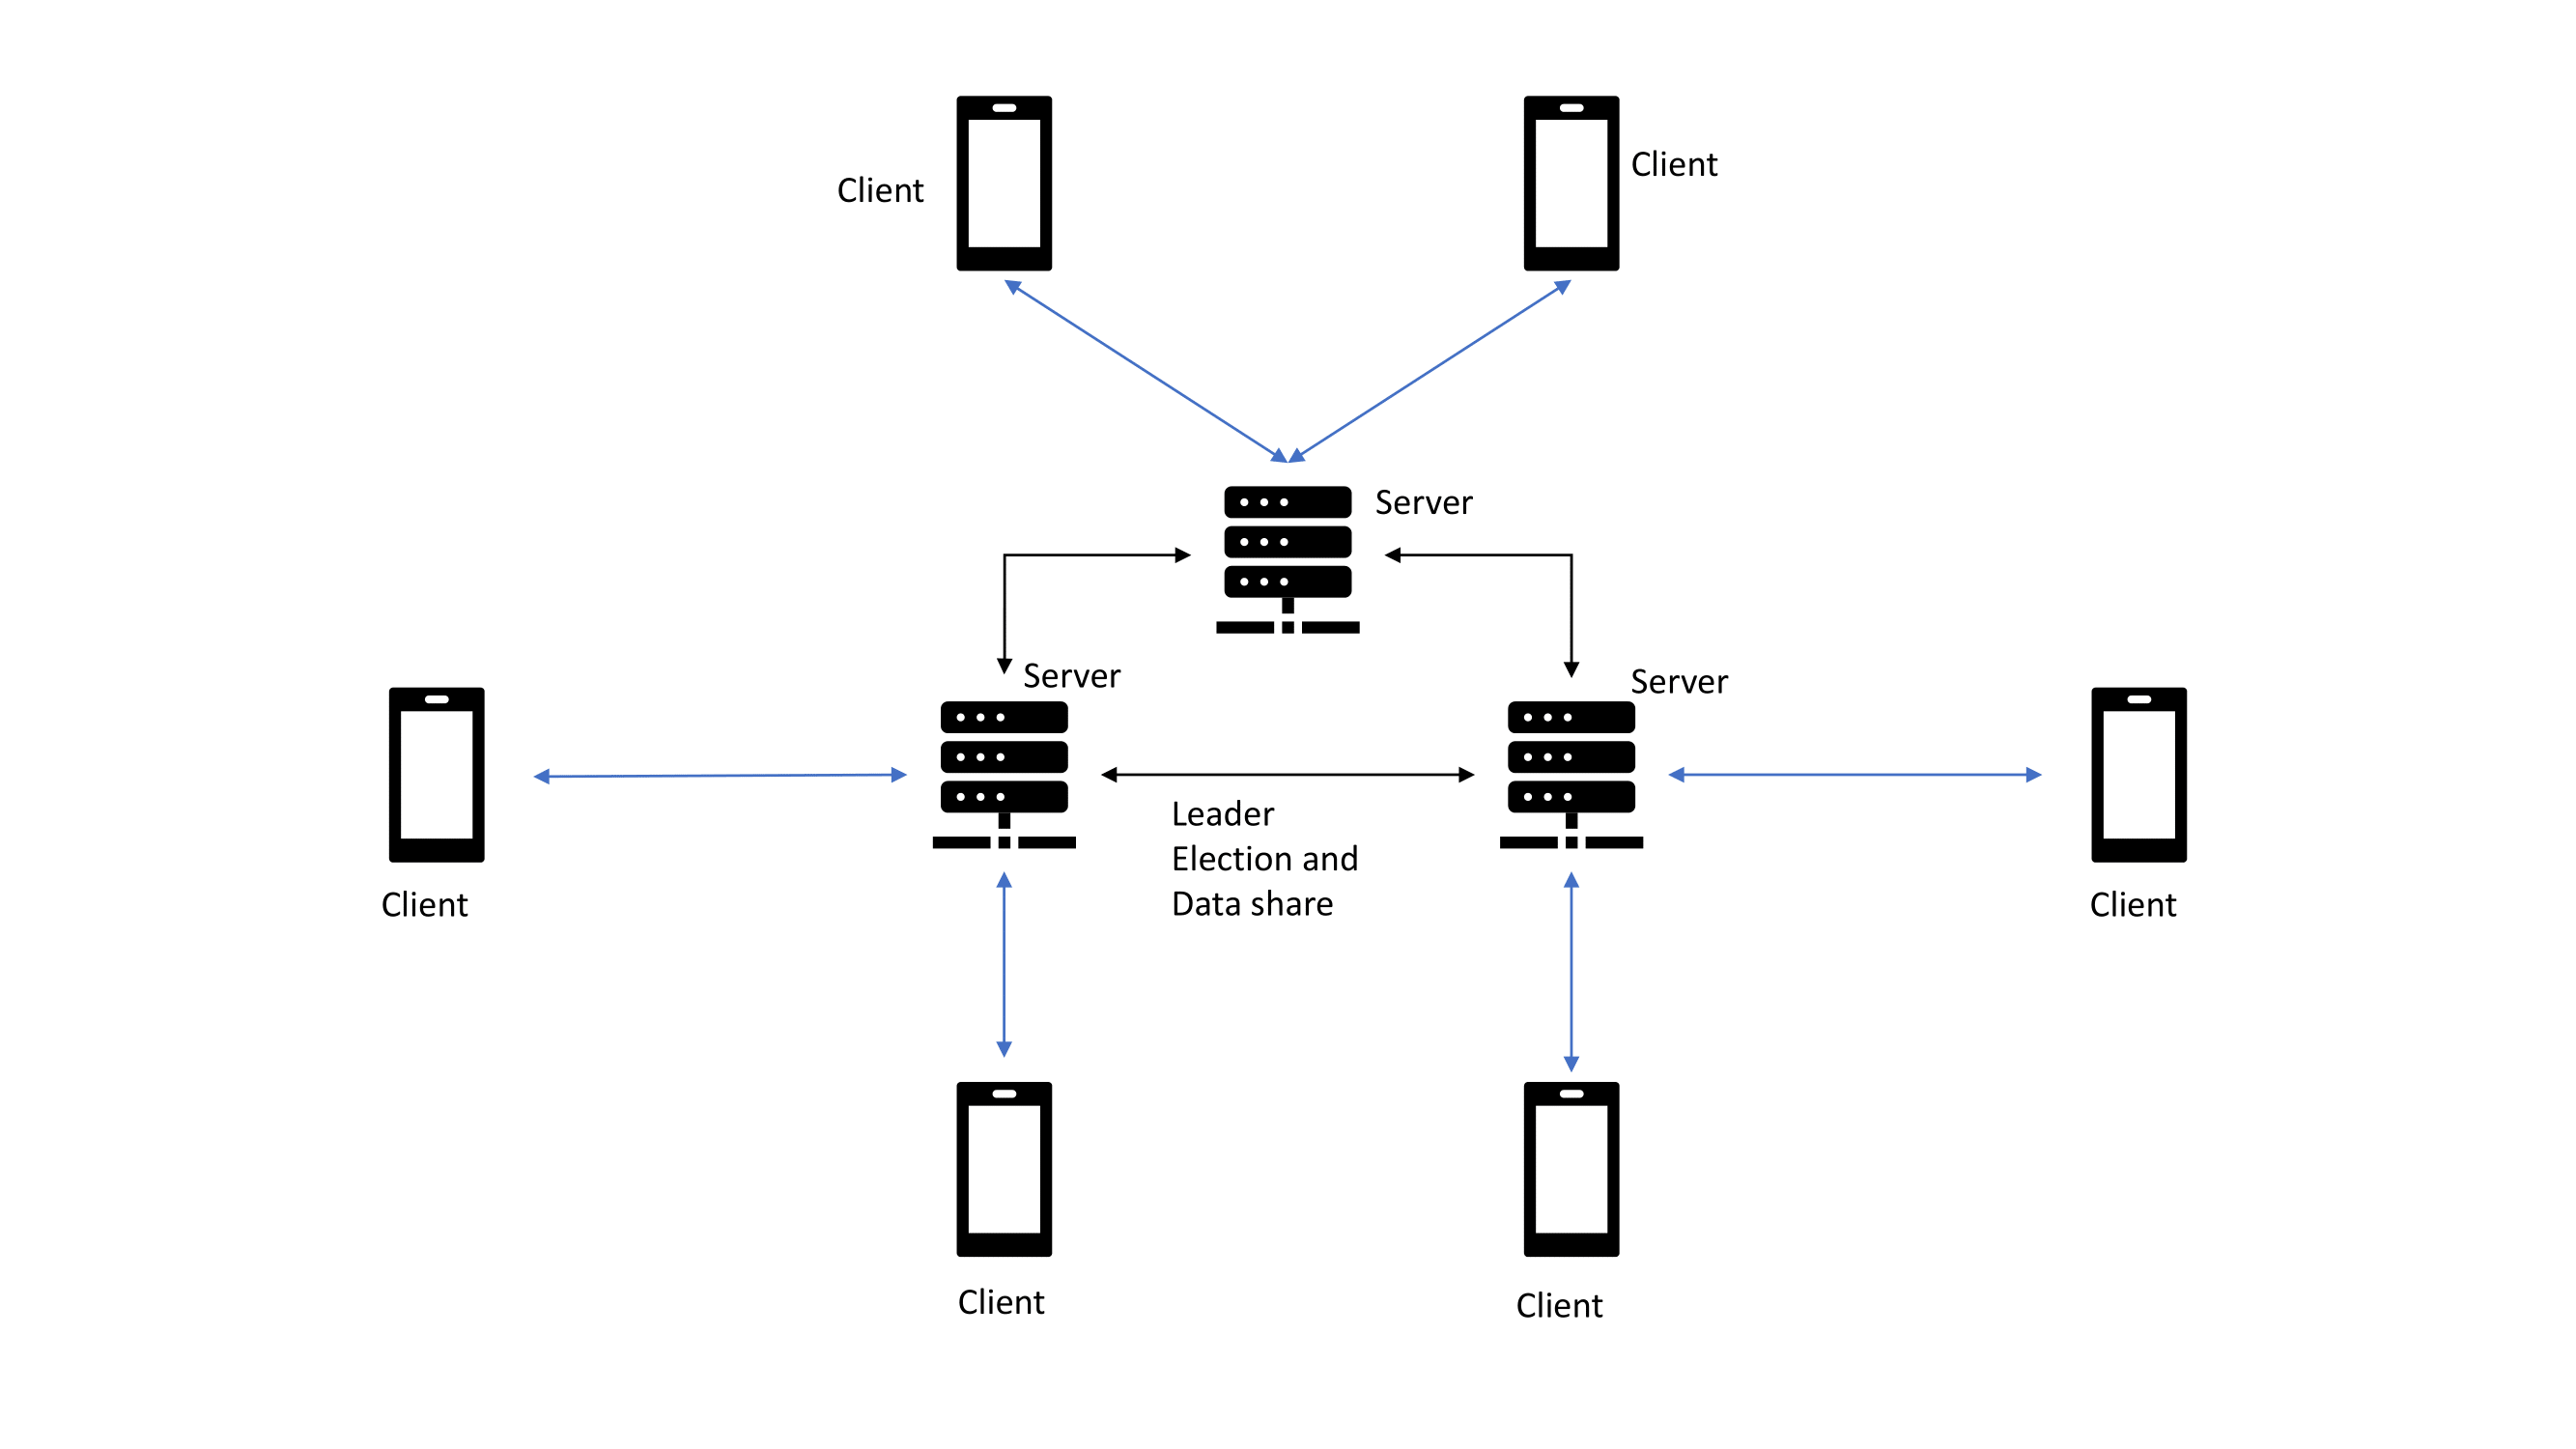
\includegraphics[width=\textwidth]{images/Architecture.png}
\caption{Architecture showing the system interaction.} \label{fig1}
\end{figure}



%
% ---- Bibliography ----
%
% BibTeX users should specify bibliography style 'splncs04'.
% References will then be sorted and formatted in the correct style.
%
% \bibliographystyle{splncs04}
% \bibliography{mybibliography}
%
%\begin{thebibliography}{8}
%\end{thebibliography}
\end{document}
